\documentclass{article}
\usepackage[utf8]{inputenc}
\usepackage{graphicx}
\usepackage{amsmath }
\usepackage{amssymb}
\usepackage{subcaption}
\usepackage{float}
\usepackage{mathtools}
\setcounter{section}{0}


\usepackage{cleveref} %referencing figures, equations and tables
\crefformat{figure}{Figure.~#2#1#3}
\crefformat{equation}{Eq.~#2#1#3}
\crefformat{table}{Table.~#2#1#3}
\crefformat{appendix}{Appendix.~#2#1#3}
\crefformat{section}{Section.~#2#1#3}

\title{Numerical Study of the Axial Impact of a Rigid Mass Against an Elastic Cantilever Beam}
\author{Amir Baharvand }
\date{}

\begin{document}

\maketitle

\section{Introduction}
The axial impact of a rigid mass and an elastic cantilever beam is a classical problem. While the problem is discussed by several authors, the original solution is attributed to Saint-Venant. Todhunter, Isaac and Pearson \cite{Todhunter1893}, Graff \cite{graff1975} and Goldsmith \cite{goldsmith2001} used the d'Alembert solution to wave equation together with the forward and backward wave equation to find the displacement field for different time intervals. Timoshenko and Goodier \cite{timoshenko1970} used the equation of motion for various time increments. In the following, the analytical solution is not provided and only a brief introduction is presented. \\

The present report aims to provide a comparison between the analytical and numerical solution of the impact of a rigid mass and an elastic beam fixed at one end and is motivated by the previous work of Escalona \emph{et.al.}\cite{Escalona1999}. This report is divided into two parts. The first part discusses the analytical solution and development of some basic mathematical equations. In the second part, ANSYS Explicit Dynamics and LS-DYNA are utilized for the numerical simulation of the problem. \\

\section{Analytical Solution}
\subsection{Problem formulation}
A schematic of the rigid mass and the elastic beam is depicted in \cref{fig:problem_formulation}. The mass has an initial velocity, $v_0$, and approaches the elastic beam in the positive direction of the $x$-axis while the elastic beam with a mass similar to the rigid body, $m$, Young's modulus, $E$, cross-sectional area, $A$, length, $l$ is at rest. The beam is also fixed at the right end ($x=l$) and is free at $x$=0.

\begin{figure}[H]
    \centering
    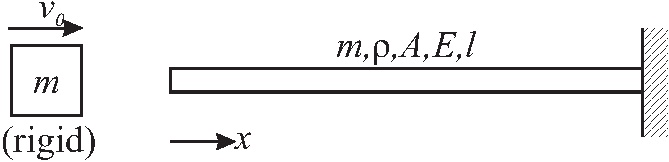
\includegraphics[width = 0.6\textwidth ]{figures/problem.pdf}
    \caption{The problem geometry and coordinate system.}
    \label{fig:problem_formulation}
\end{figure}

\subsection{Assumptions}
The following assumptions are made in developing the analytical solution.

\begin{enumerate}
    \item The mass is assumed to be rigid and the beam is elastic.
    \item The beam is long enough so that the one-dimensional wave equation is applicable.
    \item At the time of impact, all the rigid body velocity is transferred to the beam.
    \item The displacements are assumed to be infinitesimal.
    \item No friction is assumed between the mass and beam. In addition, the contact is assumed to be perfect.
    \item The effect of lateral inertia due to Poisson's ratio is disregarded. Furthermore, the vibration of the beam is neglected.
\end{enumerate}

\subsection{Discussion on the Analytical Solution}\label{sec:analytic_sol}
Due to the impact of the rigid mass with the elastic beam, a compressive stress wave, $\sigma_0$ is generated which propagates towards the positive $x$-direction. The third assumption states that after impact, the beam obtain the same velocity as the rigid mass that is

\begin{equation}
    \sigma_0 = \rho c v_0
    \label{eq:sigma_0}
\end{equation}

where $c$ is the wave propagation velocity. Due to the contact of two bodies, contact stress is generated, $\sigma(t)$, which can be calculated from the equation of motion.

\begin{equation}
    m\frac{\text{d} v(t)}{\text{d} t} = -\sigma(t) A
    \label{eq:eom}
\end{equation}

The negative sign indicates compressive stress. One can correlate the stress and velocity via

\begin{equation}
    \sigma(t) - \sigma(t_0) = \rho c [v(t) - v(t_0)]
    \label{eq:stress_wave}
\end{equation}

where $\sigma(t_0)$ and $v(t_0)$ are the stress and velocity before the impact. Since the beam is at rest at $t$=0, the above equation reduces to $\sigma(t) = \rho c v(t)$. Replacing $v(t)$ from the former line and $m/A$ with $M$ in combination with \cref{eq:eom} results in the following differential equation.

\begin{equation}
    \frac{M}{\rho c} \frac{\text{d} \sigma(t)}{\text{d} t} = -\sigma(t)
    \label{eq:ode}
\end{equation}

Solving \cref{eq:ode} with the initial condition from \cref{eq:sigma_0} gives

\begin{equation}
    \sigma(t) = \sigma_0 e^{-\textstyle\frac{\rho c}{M}t}
    \label{eq:stress_wave_sol}
\end{equation}

which implies a decreasing behavior in the generated stress (see \cref{fig:stress_wave_schematic}) \\

\begin{figure}[ht]
    \centering
    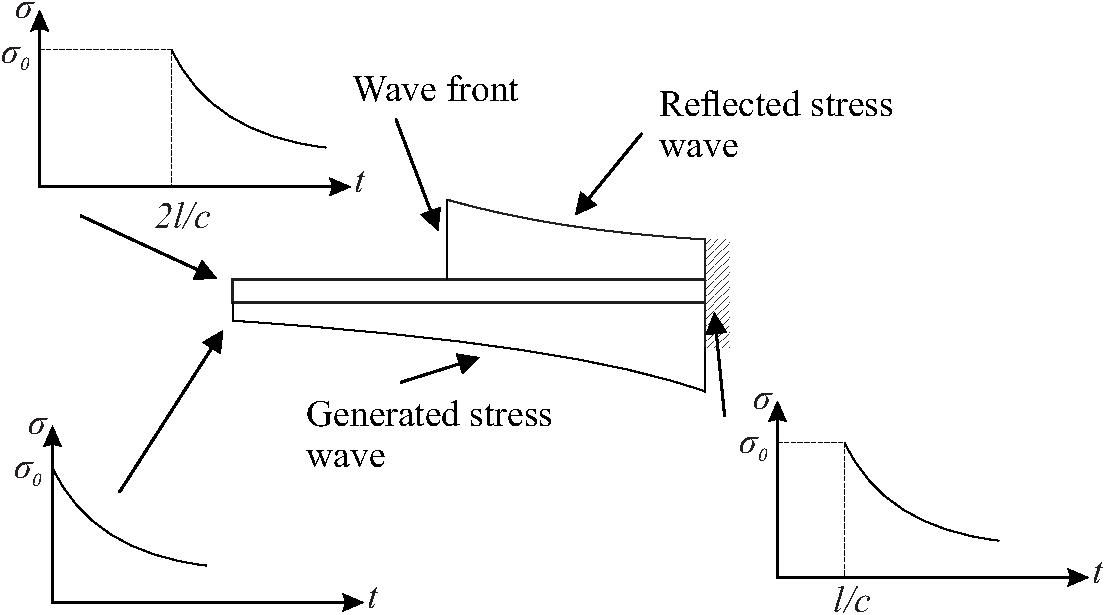
\includegraphics[width = 0.9\textwidth ]{figures/stress_wave_schematic.pdf}
    \caption{Illustration of the compressive stress waves (generated and reflected) during the first fundamental period.}
    \label{fig:stress_wave_schematic}
\end{figure}

Let $T$ be the fundamental period that is the time required for the stress wave to travel through the beam and reflect ($T=2l/c$). As soon as the stress wave arrives at the fixed boundary ($t=T/2$), it reflects as another compressive stress (2$\sigma_0$). At this instance, the contact stress can be calculated by setting $t=l/c$ in \cref{eq:stress_wave_sol}. At $t=T$, the total stress is increased by $2\sigma_0$. This jump in the total stress occurs for $nT, n = 2, 4 , ...$ intervals; thus, enforcing to update the total stress equation at each fundamental period, $T$. After the first interval, the wave reflects as another compressive wave due to the existence of the rigid mass which resembles a fixed boundary. Consequently, the compressive wave is simply the generated wave from the previous time interval with a delay $T$. Finally, the total stress is the sum of the current stress and previous stress at $t=t-T$. Denoting the value of total stress at each interval by $s$ 

\begin{equation}
    \sigma = s_n(t) + s_{n-1}(t-T)
\end{equation}

The velocity is (see \cref{eq:stress_wave})

\begin{equation}
    v = \frac{1}{\rho c} [s_n(t) - s_{n-1}(t-T)]
\end{equation}

where $n$ designates the intervals.

\section{Numerical Analysis}
\subsection{Numerical Model}
The mass and beam are modeled in ANSYS DesignModeler. The elastic beam material properties are listed in \cref{tab:mat_prop} and the mass is modeled as a rigid body. The fixed boundary is applied at the end of the beam and the beam displacements are limited in the $x$ and $y$ directions (see \cref{fig:mesh_quality}). A friction-less contact is defined between two bodies and the solver is set to Lagrangian. The element type is linear as the solver does not allow to choose a quadratic element. An initial velocity of 1m/s is defined for the mass.

\begin{table}[H]
    \centering
    \caption{Mechanical properties of the rigid mass and elastic beam.}
    \begin{tabular}{l c c c c} \hline
        Property & Symbol & Unit & Value & Attribution \\ \hline
        Density & $\rho$ & kg/m$^2$ & 7900& Mass/Beam \\
        Length & $l$ & m & 0.3 & Beam \\
        Young's modulus & $E$& Pa & 2.1E11 & Beam \\
        Poisson's ratio & $\nu$ & - & 0.3 & Beam \\
        Mass & $m$ & kg & 2.133 & Mass/Beam \\
        Area & $A$ & m$^2$ & 9E-04 & Beam \\ \hline
    \end{tabular} 
    \label{tab:mat_prop}
\end{table}

\begin{figure}[H]
    \centering
    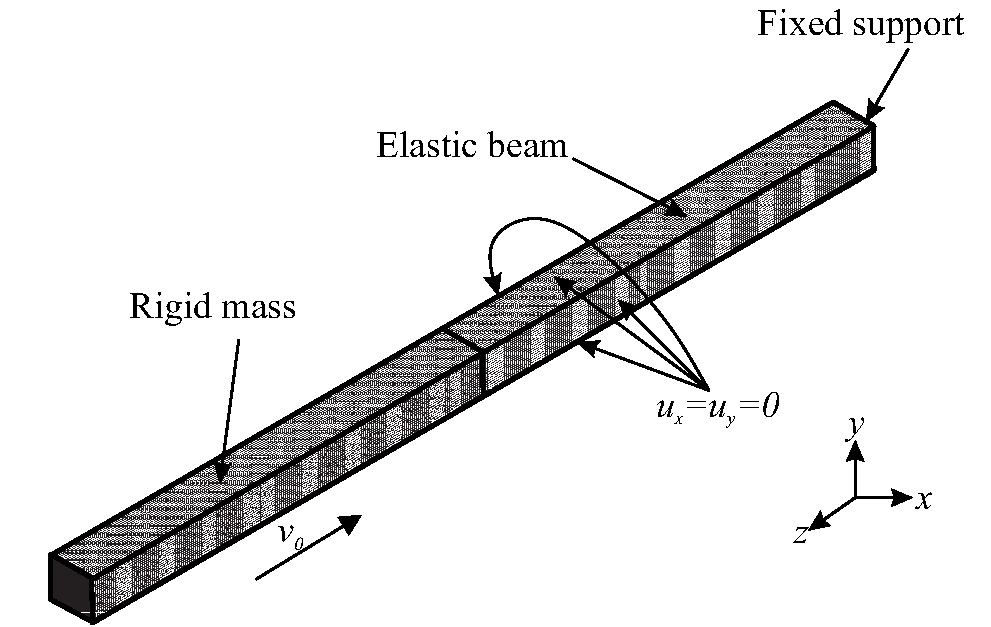
\includegraphics[width = 0.7\textwidth ]{figures/mesh_quality.pdf}
    \caption{The numerical model.}
    \label{fig:mesh_quality}
\end{figure}

\subsection{Mesh Study}
To achieve a robust numerical model, a mesh convergence study based on the area under the curve of stress-time from the initiation of contact to $t$=1.551E-05s is performed and compared to the theoretical value from \cref{eq:stress_wave_sol}. The absolute error is calculated from below. 

\begin{equation}
    \text{Error[\%]} = \frac{\sigma_1 - \sigma_2}{\sigma_2} \times 100
    \label{eq:error}
\end{equation}

where $\sigma_1$ and $\sigma_2$ denote the analytical and numerical values of stress, respectively. \cref{tab:mesh_convergence} summarizes mesh number, $N$, size and the absolute error. The stress plots from the numerical method are given in \cref{fig:stress_distribution}. \cref{fig:mesh_convergence} show that the mesh converges to below 1.5\% for $N$=160000\footnote{Opting for a finer mesh less than the last row in \cref{tab:mesh_convergence} causes the solver to crash due to limited RAM resources. Increasing the RAM in the \texttt{input.k} file and using the LS-Run and Mechanical APDL Product Launcher tools does not help.}. 

\begin{figure}[!]
    \centering
        \begin{subfigure}{0.65\textwidth}
            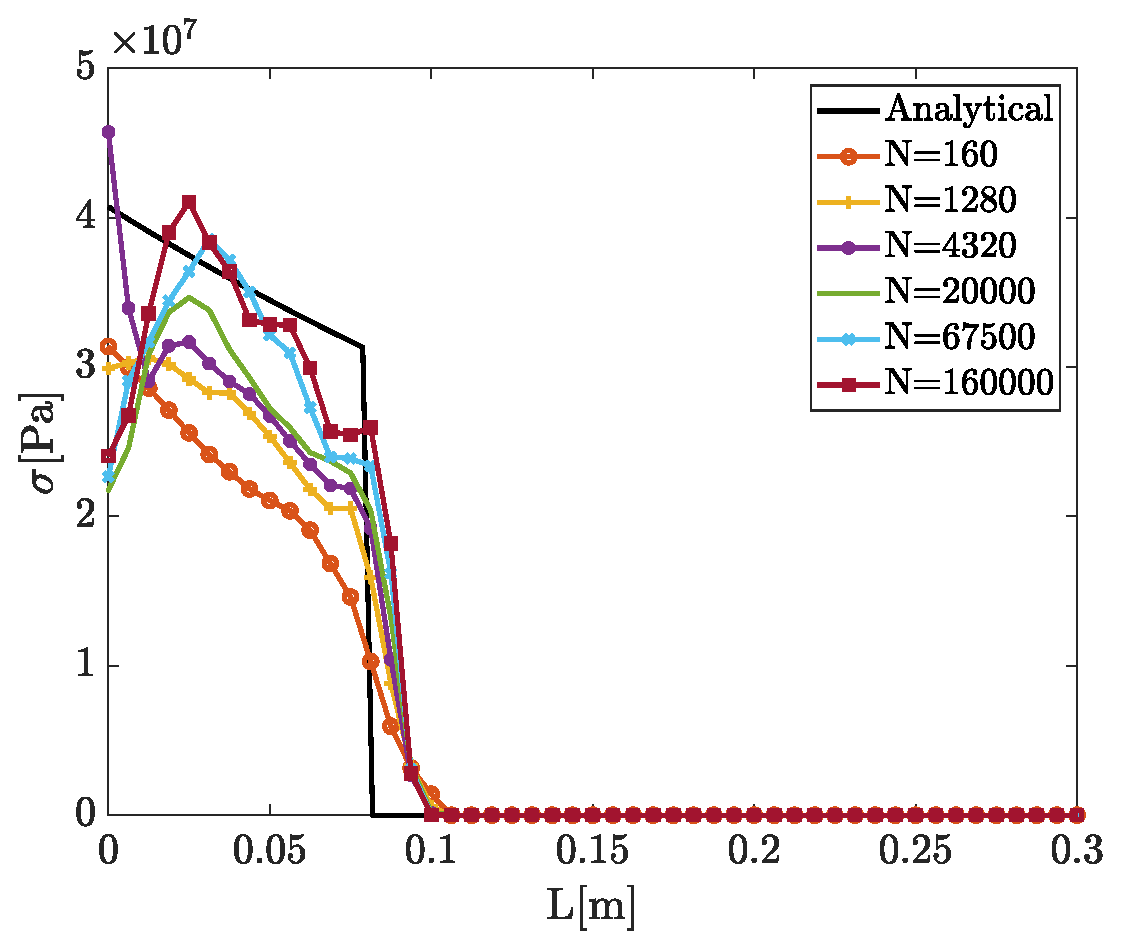
\includegraphics[width=1\linewidth]{figures/stress_mesh_study.eps} 
            \caption{}
            \label{fig:stress_distribution}
        \end{subfigure}
        
        \begin{subfigure}{0.7\textwidth}
            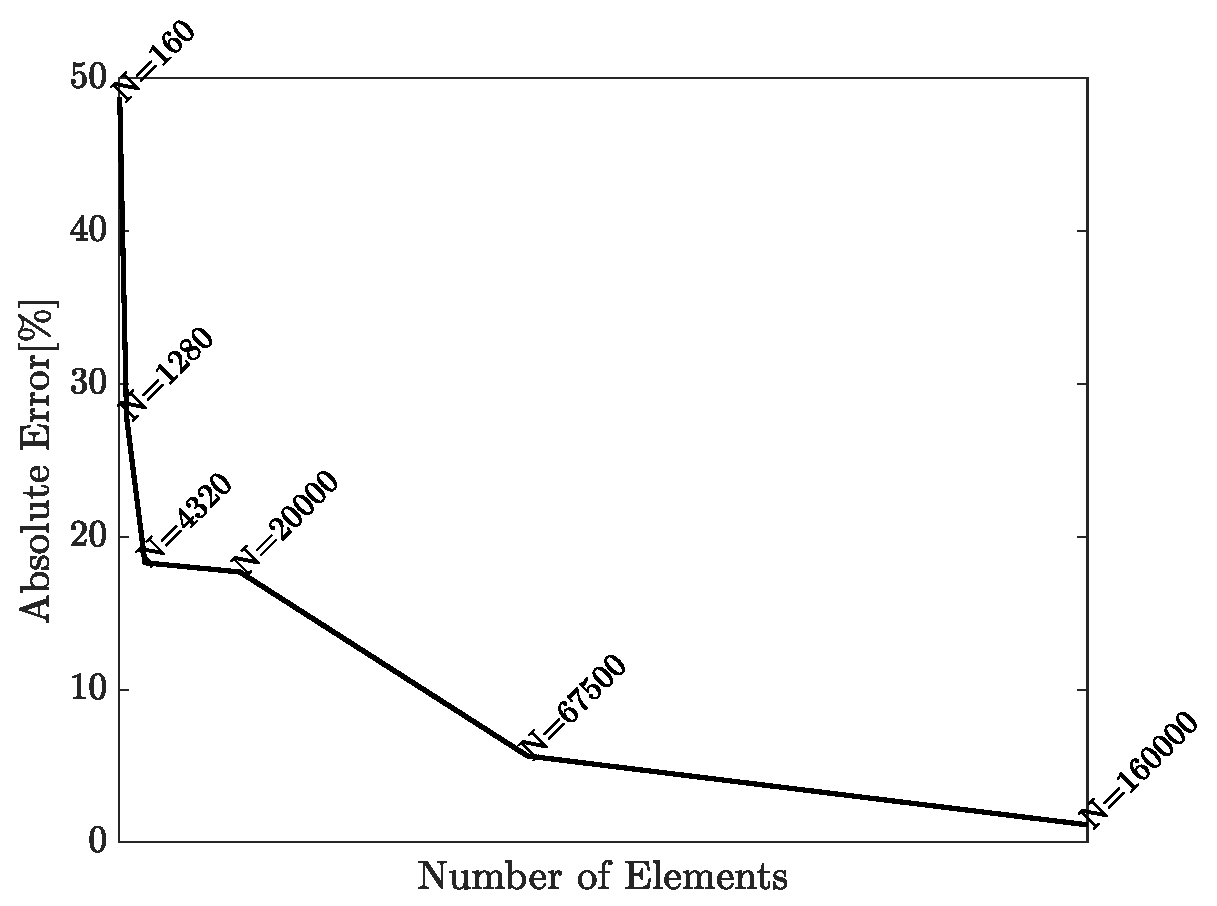
\includegraphics[width=1\linewidth]{figures/mesh_study.eps} 
            \caption{}
            \label{fig:mesh_convergence}
        \end{subfigure}
    \caption{(a) Stress wave distribution along the beam coordinate at $t$=1.551E-05s for the different numbers of elements. (b) Mesh convergence plot.}
    % \label{}
\end{figure}

\begin{table}[H]
    \centering
    \caption{Numerical model mesh information.}
    \begin{tabular}{l c c} \hline
        Number of elements ($N$) & Smallest dimension [m] & Absolute error[\%] \\ \hline
        160 & 0.0150 & 48.72 \\
        1280 & 0.0075 & 27.86 \\
        4320 & 0.0050 & 18.30 \\
        20000 & 0.0030 & 17.70 \\
        67500 & 0.0020 & 5.66 \\
        160000 & 0.0015 & 1.15 \\ \hline
    \end{tabular} 
    \label{tab:mesh_convergence}
\end{table}

\subsection{Results and Discussion}
The displacement-time plot of the free-end of the elastic beam ($x$=0) is shown in \cref{fig:displ}. The numerical result follows the analytical solution curve until $T/2$; however, after this time, the difference between the two plots increases. It may seem that the reflected stress wave produces errors in calculating the displacement. \\

\begin{figure}[ht]
    \centering
    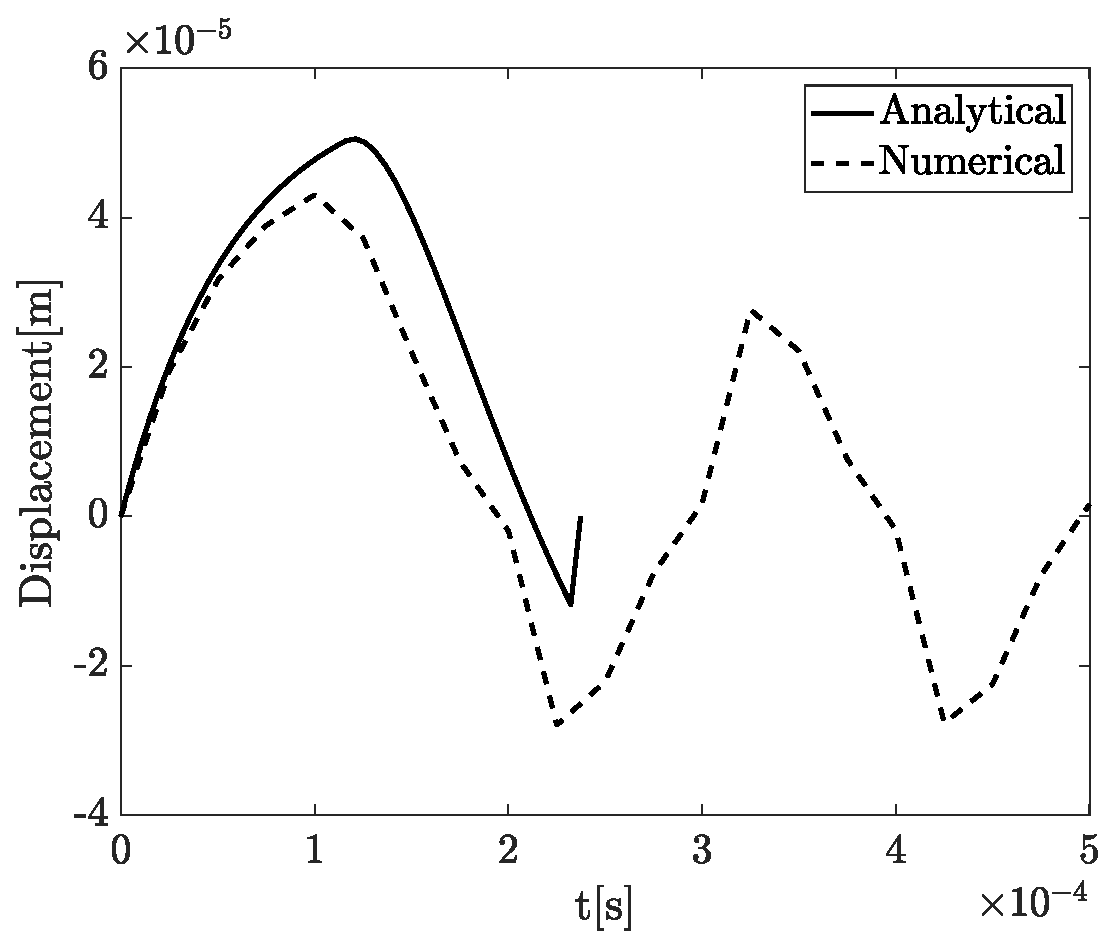
\includegraphics[width = 0.6\textwidth ]{figures/displacement.eps}
    \caption{Displacement at the free-end of the beam ($x$=0) for various time increments ($t_{max}=T$).}
    \label{fig:displ}
\end{figure}

The stress distribution along the beam coordinate is plotted in \cref{fig:stress_t1_t3} for three time cases (the first two, before $T/2$ and the last after $T/2$). These results are extracted from LS-DYNA as ANSYS Explicit Dynamics was not able to predict the falling behavior of the stress. Overall, the numerical model can predict the behavior of the stress distribution except for \cref{fig:sigma_t2}. Due to the determination of stress from the displacement field in the finite element method (FEM) and good agreement between the analytical and numerical results in the displacement plot (\cref{fig:displ}), the author has no clear explanation for the stress plot in \cref{fig:sigma_t2}. It is also evident from the plots that the number of mesh and time increment play a key role in the numerical result (see \cref{fig:sigma_t1} and \cref{fig:sigma_t2}) as the first value of stress at $t$=0 is almost half of the analytical solution then suddenly jumps to its corresponding analytical value. \\ 

\begin{figure}[ht]
        \begin{subfigure}{0.5\textwidth}
            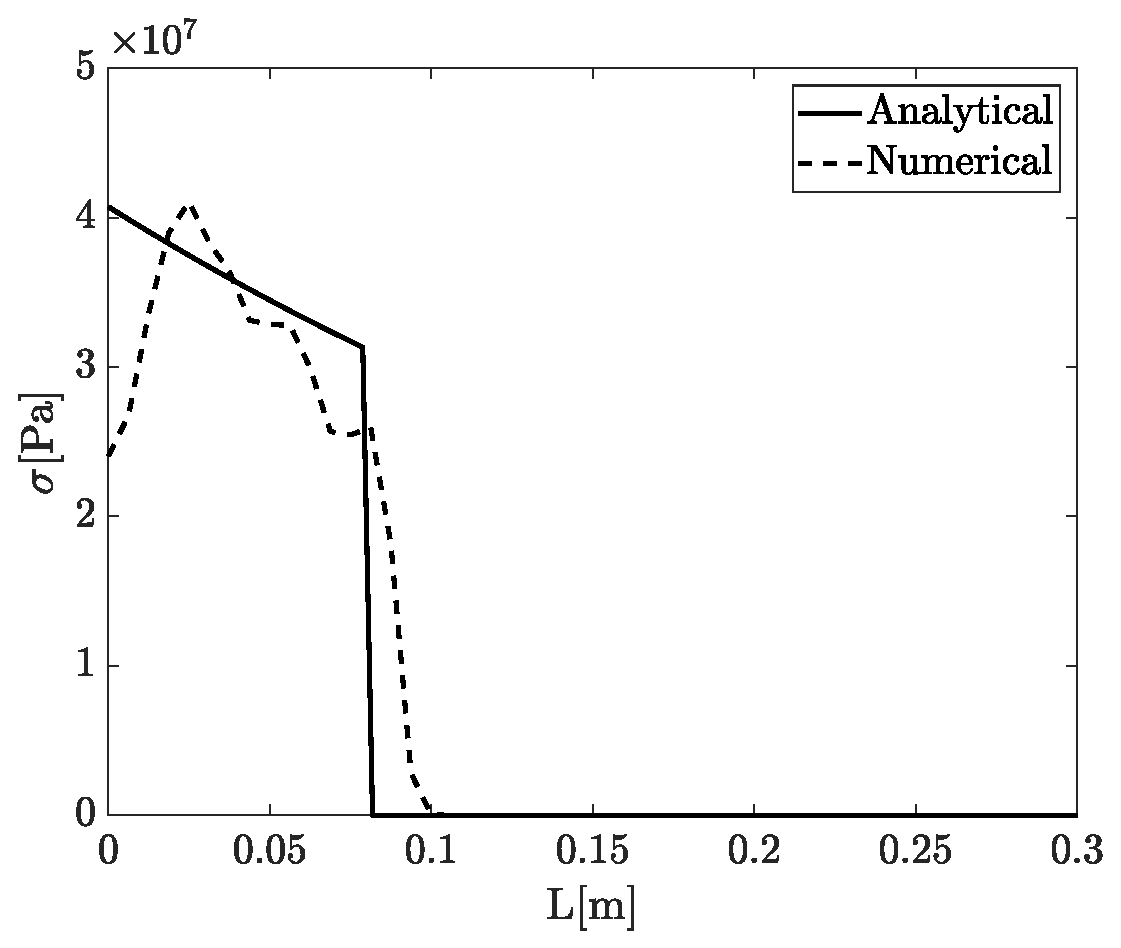
\includegraphics[width=1\linewidth, height=0.8\linewidth]{figures/stress_t1.eps} 
            \caption{$t$=1.551E-05s}
            \label{fig:sigma_t1}
        \end{subfigure}
        \begin{subfigure}{0.5\textwidth}
            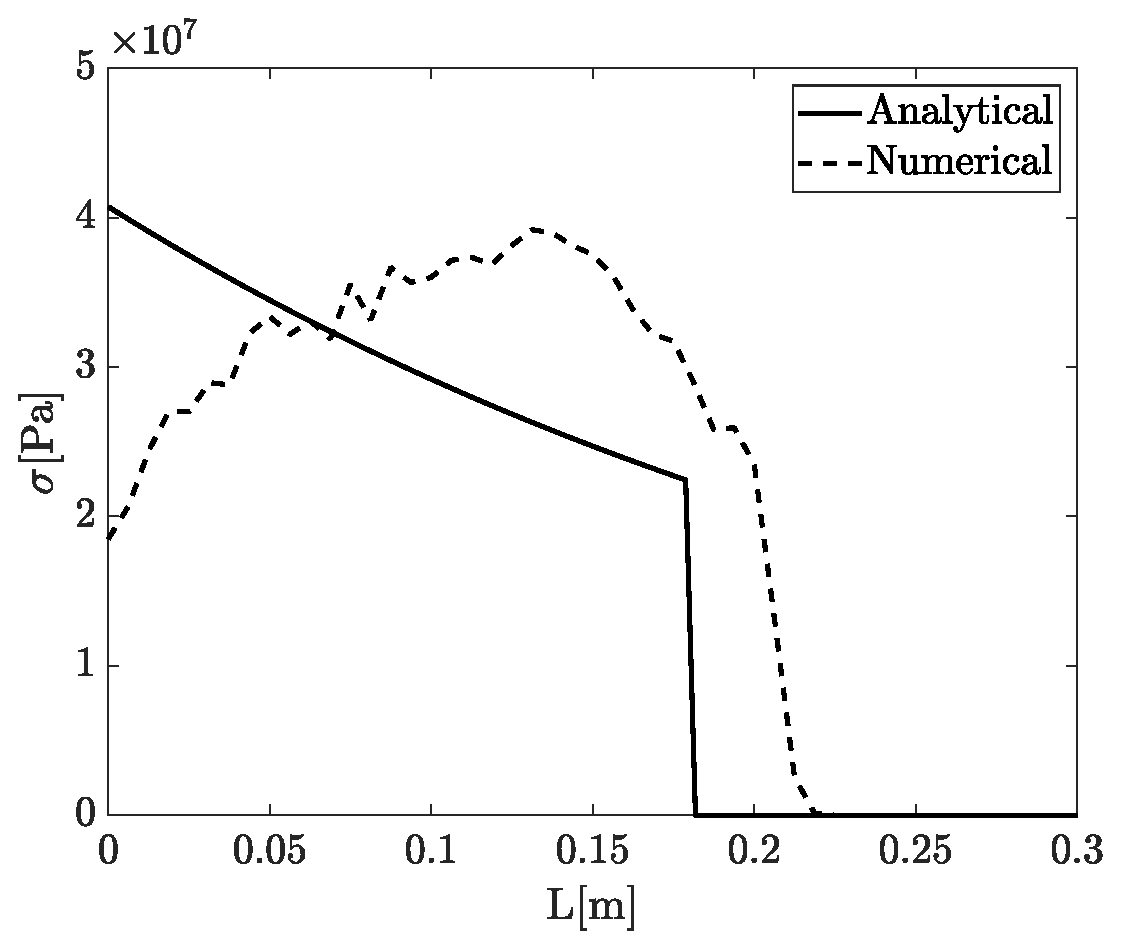
\includegraphics[width=1\linewidth, height=0.8\linewidth]{figures/stress_t2.eps} 
            \caption{$t$=3.49E-05s}
            \label{fig:sigma_t2}
        \end{subfigure}
        \begin{subfigure}{0.5\textwidth}
            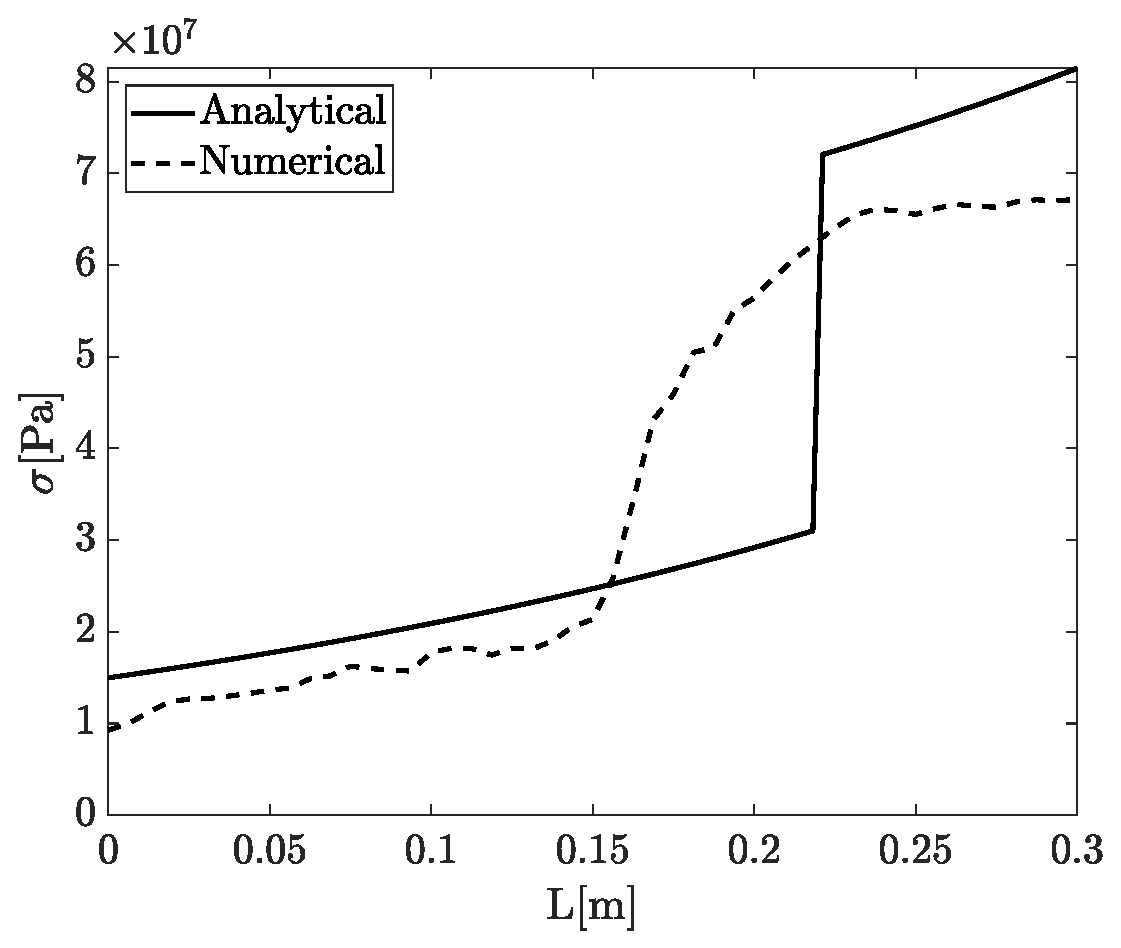
\includegraphics[width=1\linewidth, height=0.8\linewidth]{figures/stress_t3.eps} 
            \caption{$t$=7.370E-05s}
            \label{fig:sigma_t3}
        \end{subfigure}
    \caption{Stress wave distribution along the beam coordinate for three time cases.}
    \label{fig:stress_t1_t3}
\end{figure}

\cref{fig:contact_pressure} shows the distribution of contact pressure. Once more, the importance of a finer mesh is visible for the numerical result at $t$=0 and 1.25E-04s ($t=T$). At about $t=T$ the reflection of the stress wave from the rigid mass is obvious (see section \ref{sec:analytic_sol}).

\begin{figure}[H]
    \centering
    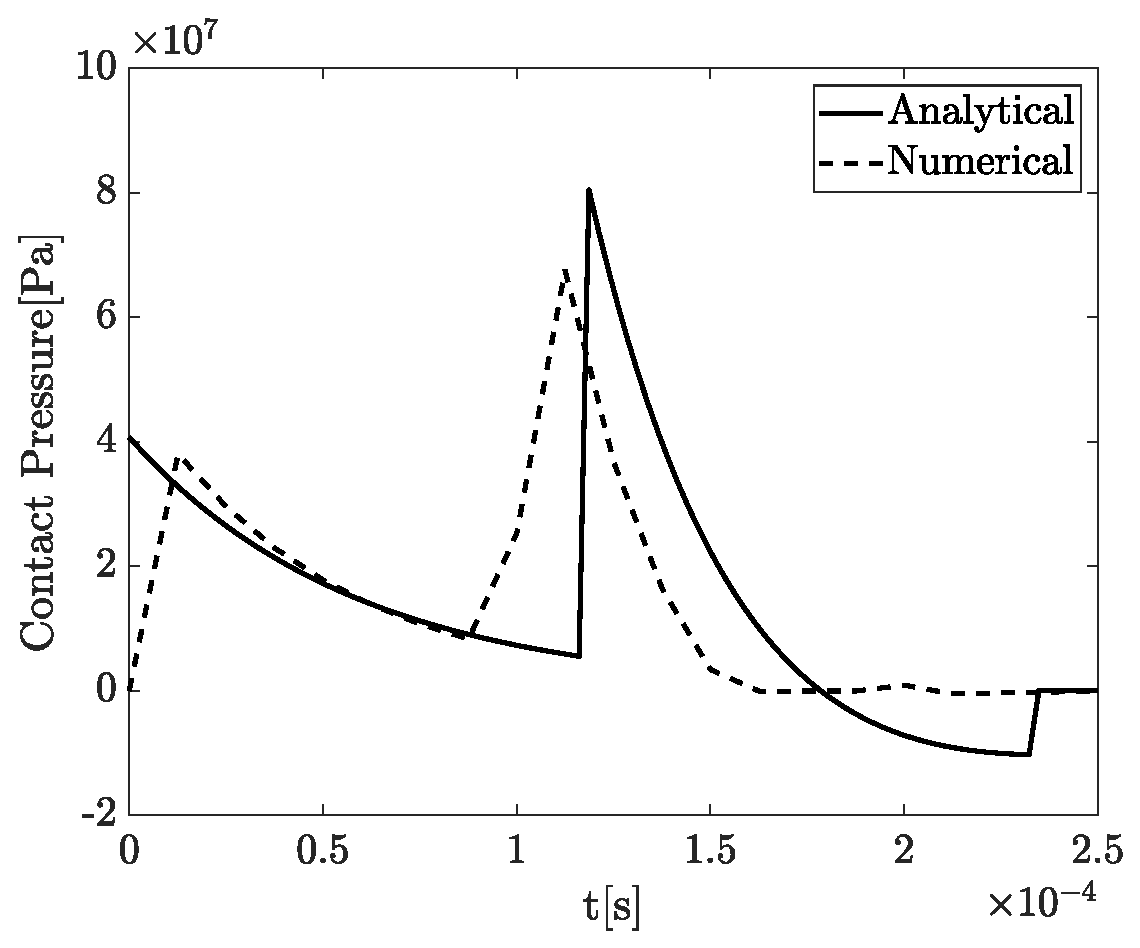
\includegraphics[width = 0.6\textwidth ]{figures/contact_pressure.eps}
    \caption{Contact pressure at the free-end of the beam ($x$=0) for various time increments ($t_{max}=2T$).}
    \label{fig:contact_pressure}
\end{figure}

The reaction stress (\cref{fig:reaction_stress}) is calculated from the reaction forces at the fixed boundary of the beam and then divided by the beam area. The numerical result shows a good agreement with the analytical until the end of the first period. The reaction stress is zero up to the arrival of the stress wave, generated at the free-end, then rises to 2$\sigma_0$ due to the reflection of the stress wave. After $2T$, the numerical model fails to characterize the reaction stress due to the previously-mentioned reasons. \\ 

\begin{figure}[H]
    \centering
    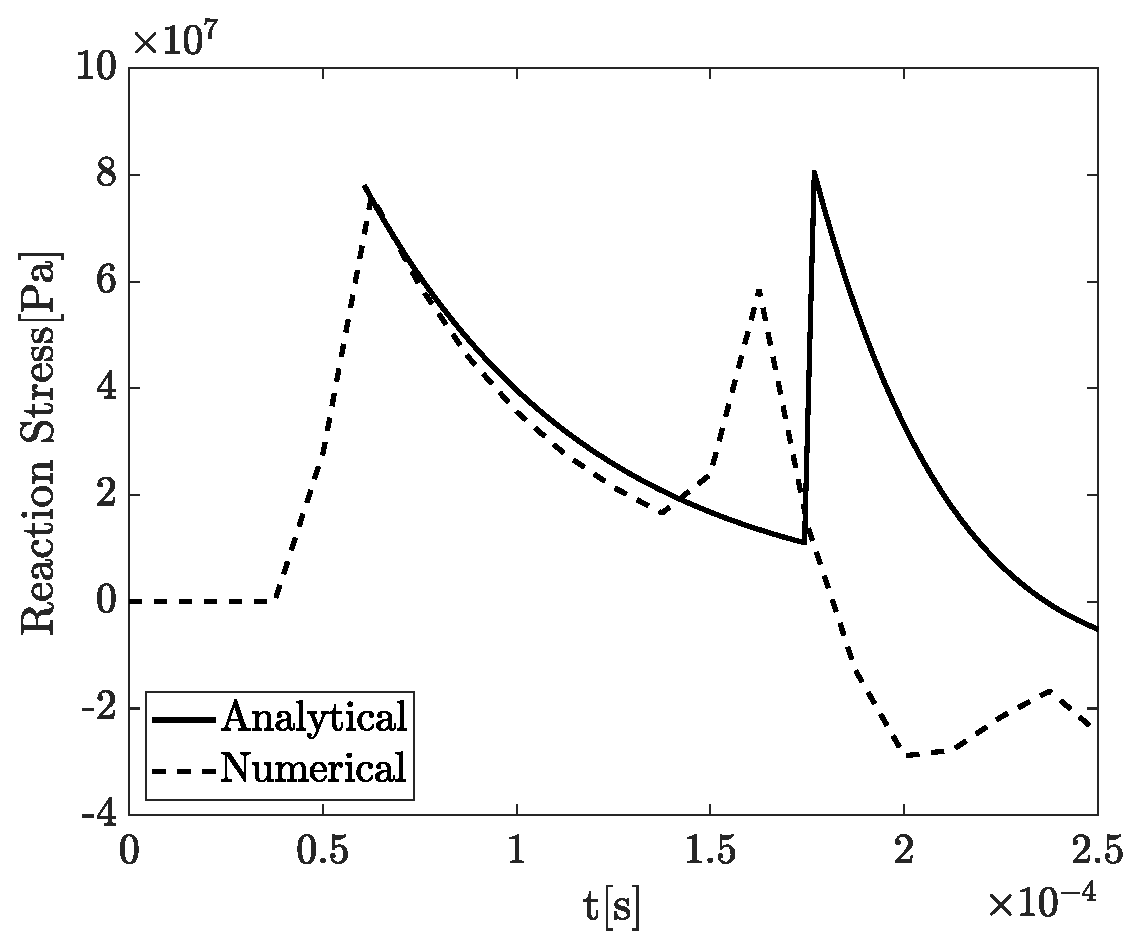
\includegraphics[width = 0.6\textwidth ]{figures/reaction_stress.eps}
    \caption{Reaction pressure at the fixed-support ($x=l$) for various time increments ($t_{max}=2T$).}
    \label{fig:reaction_stress}
\end{figure}

\section{Conclusion}
A brief introduction on the axial impact of a rigid mass against an elastic cantilever beam is provided. A numerical model is also developed and the results are compared to the analytical model. It is shown that the numerical model underestimates the displacement and stress which can be a result of the limited degrees of freedom in the finite element method (FEM). FEM is incapable of predicting the correct displacement of a multi degree-of-freedom system as the degrees of freedom in a numerical model is limited. In addition, the importance of the mesh convergence study with a fine mesh at the contact surfaces along with smaller time increments is emphasized.


\newpage
\bibliography{ref}
\bibliographystyle{ieeetr}

\end{document}